%%%%%%%%%%%%%%%%%%%%%%%%%%%%%%%%%%%%%%%%%%%%%%%%%%%%%%%%%%%%%%%%%%%%%%%%%%%%%%%%%%%%%%%%%%%%%%%%%%%%%%%%%%%%%%%%%%%%%%%%%%%%%%%%%%%%%%%%%
% Abstract: dar uma idéia dos principais resultados encontrados. 
% Introdução: cenário, motivacao, problema, solucoes atuais, escopo do artigo, lista de contribuicoes, organizacao do resto do artigo. 
% Trabalhos Relacionados: fazer uma das duas coisas a seguir (ou as duas): 
%	a) quando citar uma ou um grupo de referencias relacionado an um tema especifico, conclua o paragrafo mostrando a diferenca para a proposta a ser descrita. 
%	b) no final da secao, compile todas as diferenças e deixe explicito as contribuicoes novamente.
% Metodologia: coloque uma figura para ilustrar todo o processo de coleta e analise. coloque numa tabela (ou mais de uma) a descricao das metricas de interesse, alem dos fatores e niveis selecionados em outra tabela. explique o motivo desses fatores influenciarem as metricas de interesse.
% Conclusão: evite apresentar os resultados mais fáceis de concluir. bons revisores olham o casamento do que vc escreve no abstract/introdução com a conclusao, então mantenha coerente an introdução com a conclusão. Em geral, resultados que sao aparentemente obvios - nao eram até vc mostrar :) - enfraquecem as outras contribuicoes. p.ex, "Os resultados mostraram que o MapReduce apresenta uma boa solução para utilizar computadores comuns para obter alta capacidade de processamento e lidar com an análise massiva de tráfego de rede." pode ser reformulado ou retirado da conclusao. 
\chapter{Offline Mode for Corporate Mobile Client Security Architecture}
\label{ch:mobile}

\begin{quotation}[]{Confucius}
Life is really simple, but we insist on making it complicated.
\end{quotation}

\section{Introduction}
\label{sec_intro}
Cloud computing is a new rapidly evolving paradigm in the world of distributed networking and computation. The basic features of the cloud environment is providing the elastic, on-demand and secure services for the end-users. While the first two requirements are rather well conceptualized and supported by the majority of the cloud platforms in use, security is a serious concern of the cloud providers and governmental organizations as well as academia and research community \cite{csa2016,higashi2015,gartner2015}. Although for the small and medium-sized enterprises (SME) the cloud environment is often the most cost-effective and easily scalable solution, the security and privacy of the sensitive data in cloud platforms are also not fully conceptualized leading to obscure and incomplete security paradigms and solutions.

A common practice to provide a cloud solution with stable security is to use a specific type of cloud service, such as Cloud Access Security Broker (CASB) or Cloud Access Control (CAC). These services are specifically designed to bring security at a single access point and provide the coordination of the most important security measures. Gartner \cite{skyhigh2015} estimates that such systems will be used by 85 \%  of companies by 2020. The reason for this is that the organization of security measures at a single control point allows to control and to monitor the level of cloud protection much more effectively. The basic features of the CASB are: discovery of cloud services, encryption along with tokenization for better search properties, access control, Data Loss Prevention (DLP) services, authentication, and auditing and alerting services \cite{lawson2015}. The protection of the confidential data, according to the standards of CASB deployment should be provided elsewhere, i.e. in transit and at the end-user, i.e. end-client, side \cite{campbell2015}.

Additional security issues and requirements have to be considered when mobile clients are actively used in corporate cloud environment \cite{yovel2014}. Today more and more organizations and enterprises are functioning in the Bring-Your-Own-Device (BYOD) paradigm. The uncontrolled usage of the mobile devices represents a serious risk to the development of secure SME cloud platforms being the bottleneck of the corporate information security system (ISS). While the enterprise cloud infrastructure based on the web interface can be protected by powerful third-party services, such as CASB and CAC, the corporate mobile client is usually light-weighted and generally less protected. 

The protection scheme used on a mobile device should be both computationally secure as well as resource-constrained due to battery power limitations \cite{khan2015cloud}. Therefore, encrypting files and generating keys on a mobile device is not considered a good solution. On the other hand, the protection schemes with good computational qualities lack the security analysis in many cases \cite{khan2014bss}. The common practice is the shadow user activities monitoring \cite{yovel2014}. However, the mobile device usage stays unprotected in all the proposed scenarios while in offline mode.

Suppose that a SME uses CASB to protect data at rest, i.e. while stored on the server-side, in transit, communicating with server, and, in use, while the mobile client is connected to the network. In this case, when the mobile client goes offline with the sensitive corporate data on board all powerful cloud-based tools cannot help and the mobile client has to secure itself with its own limited resources. Moreover, due to the resources constraint, there is a crucial difference in strategy of online and offline mode protection. For example, offline mode does not allow performing the extensive computation and encryption on the mobile device.
Observing the above described landscape, this paper outlines the concept of the offline mobile cloud security. 

This paper proposes a novel approach based on powerful cryptographic preventive methods, such as secret sharing (SSS) \cite{galibus2007} and Attribute-based Encryption (ABE) \citep{goyal2006attribute} for securing mobile clients. Moreover, our proposed approach includes the user behavior analysis based on Model Order Selection (MOS) \cite{tenorio2013greatest}, in order to detect possible threats, and to reduce the risks and the harm of the most common threats, which are the expired user misusing password and the intruder attack. The key expiration period is safely incorporated into the proposed system solution in order to enhance security. Additionally, the behavioral analysis can indicate well known malicious behaviors, their variations, as well as novel attacks, which present low or high variance in comparison to legitimate user behaviors. The main target of our proposed solution is to provide a maximum defense at the minimal resource cost.

The paper is structured as follows. Section \ref{sec_related_works} analyzes the most common security problems in the mobile cloud environment and the solutions for offline protection in the BYOD world. Section \ref{sec_the_client_security_architecture} outlines the mobile security architecture of the proposed solution. Section \ref{sec_offline_mode} presents the detailed scheme of the proposed solution to the problem of offline mobile client security. Section \ref{sec_algorithms} explains the algorithms for the core security methods: AES, ABE, SSS and MOS. Section \ref{sec_results} discusses the security proofs including the outline of adversary model, the common threat scenarios, the data modeling, the complexity analysis and dicussion of the practical implementation results. Section \ref{sec_conclusion} concludes the paper.

\section{Related works}
\label{sec_related_works}
The increasing usage of BYOD demands more sophisticated data protection services compared to ordinary computing environment. A common practice is to provide additional contextual methods apart from authentication, DLP services, and encryption, which can be at rest, in transit and in use \cite{yovel2014, khan2015cloud, khan2014survey, khan2013towards}. The contextual methods increase the security of the mobile client at a maximum level with minimum resource requirements. The most commonly used are:

\begin{enumerate}
	\item Using geolocation of the device to trace its usage;
	\item Setting up the expiration period of an app;
	\item Setting up the expiration period of client pass pin;
	\item Setting up the counter of failed tries;
	\item Secured transfer politics between apps;
	\item Restricting access to the corporate app;
	\item Restricted or prohibited offline access;
	\item Logging and auditing.
\end{enumerate}

Preventing data leakage on the mobile device is a crucial security problem. Therefore, it is necessary to take additional control and protection measures for the confidential data on the mobile devices that leave the boundaries of the organization. Generally, the most sensitive and confidential data should not be permitted to be transferred to the mobile device. However, what if the SME need to allow their employees to work on such devices and even use them on the offline mode for the convenience and traffic reducing, or even for a particular characteristic of the mobile client or the business itself?

From the theoretical point of view of this problem, there are several surveys, whose common point is the mobile cloud as a rapidly developing paradigm that poses many security and complexity problems \cite{khan2013towards, yovel2014, khan2014survey, khan2015cloud, mayrhofer2015architecture, chang2015design, xia2015tinman, kulkarni2015addressing, shila2016amcloud, heydari2016efficient}. Kulkarni and Khanai \cite{kulkarni2015addressing} discuss the most important threats related to Mobile Cloud Computing and argue that there is a need for a lightweight secure framework that provides security with minimum communication and processing overhead on mobile devices. 

An analysis of the new models of mobile cloud computing and new ways of using data storage services is presented in \cite{khan2015cloud, khan2013towards, mayrhofer2015architecture, chang2015design}. Commonly, the models and protection schemes concentrate on the encryption properties and either perform the computations on their own \cite{zhao2010trusted, yang2011provable} or use the cloud provider to off-load the cryptographic operations \cite{itani2010energy, ren2011lightweight}. Obviously, it is natural the mobile client cannot handle all operations securely without the assistance of a cloud provider, due to resources constraint and battery limitation.

The necessity to use schemes that function without putting load on a provider arises when it is desired to make the mobile client less dependent on the cloud provider, i.e. corporate client continues to provide the secure access to the sensitive data without connection to the network. As discussed in \cite{khan2015cloud}, all the currently known schemes of encryption, performing the computation, either use a cloud provider \cite{zhao2010trusted}, a third party trusted agent \cite{yang2011provable, heydari2016efficient}, a combination of both \cite{itani2010energy} or ad hoc approaches \cite{shila2016amcloud}. In some cases, they concentrate on computational complexity without taking care of user privacy and security \cite{ren2011lightweight}. Therefore, according to \cite{khan2013towards, khan2015cloud}, the state-of-the-art mobile cloud security models do not consider the problem of the offline security mode. 

In many cases the industrial providers of the mobile security API avoid the problem by completely forbidding the offline access to the protected app, i.e. SAP Mocona, which operates as a secure client wrapping layer \cite{Lelyveld2013}. Due to various constraints such as traffic load, travelling and ease of access, the SME business procedure may require such access. To the best of our knowledge, the offline mode security problem has not yet been deployed, neither in academia nor in the industry \cite{yovel2014, khan2015cloud, khan2014survey, khan2013towards}. Therefore, the main concern of this proposal is the protection of the mobile client and its data in offline mode, when the functions of data protection cannot be offloaded to a cloud or a trusted party. 

\section{The mobile security architecture}
\label{sec_the_client_security_architecture}
The approach proposed in this work describes and implements the complete lifecycle of the mobile client security infrastructure. The mobile security processes depend on the key expiry period, and are used to access the protected storage. Once the user keys expire, the user is requested to enter his valid credentials, i.e. PIN and password. The mobile client then sends the credentials to the server for verification. Once the new set of access keys is received, the user can access the protected files in the offline mode, without the access to the server. This means that no further communication with the server is needed until the key expires. 

The core set of functions and protocols can be divided into three sets of operations as shown in Figure \ref{fig:01}.

\begin{figure}[h!]
	\centering
	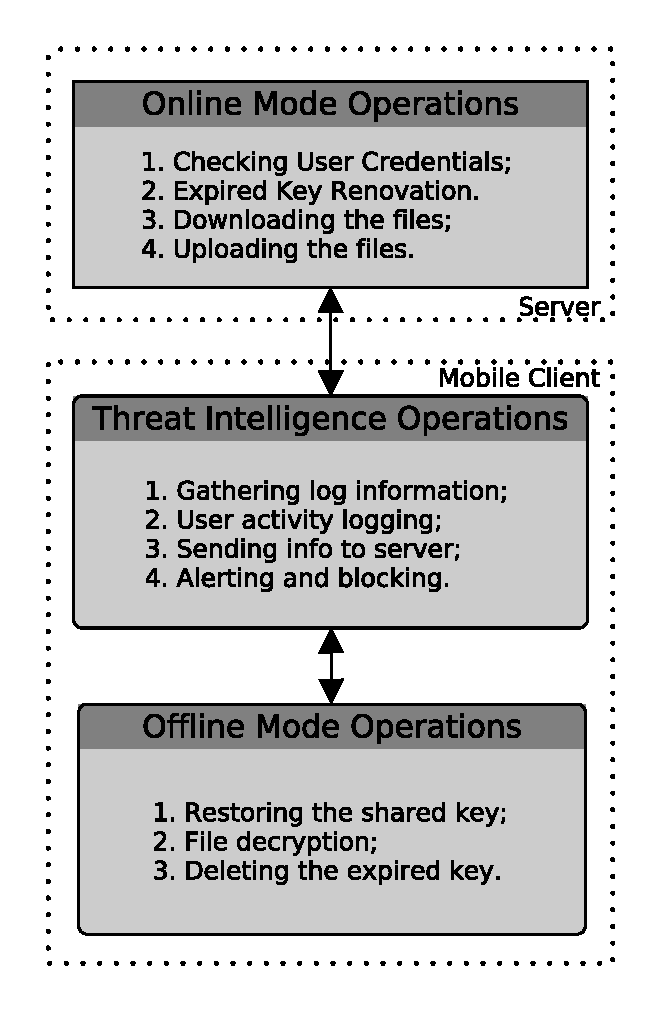
\includegraphics[width=5cm]{figures/fig01.eps}
	\caption{The core set of functions and protocols of the mobile cloud security infrastructure}
	\label{fig:01}
\end{figure}

Figure \ref{fig:01} describes the mobile client protection both in online and offline mode. In online mode, the client has the possibility to connect to the server and the security of the client is enhanced by the server-backed up mechanisms. On the other hand, in offline mode the client’s security is supported by the standalone mechanisms. Additionally, the mobile client protection is enhanced by the threat intelligence unit providing the constant monitoring and analysis.

Figure \ref{fig:02} depicts the client-side protection mechanisms. The client should support 4 subsystems: i) encryption subsystem that contains the procedures of encryption and decryption; ii) storage subsystem that provides the downloaded shares and key storage protection; iii) threat intelligence unit that provides the constant monitoring, and iv) the communication subsystem. In short, all security procedures are connected to 4 groups of operations: file request and receiving; encryption and decryption; file and key storing; monitoring and analysis.

\begin{figure}[h!]
	\centering
	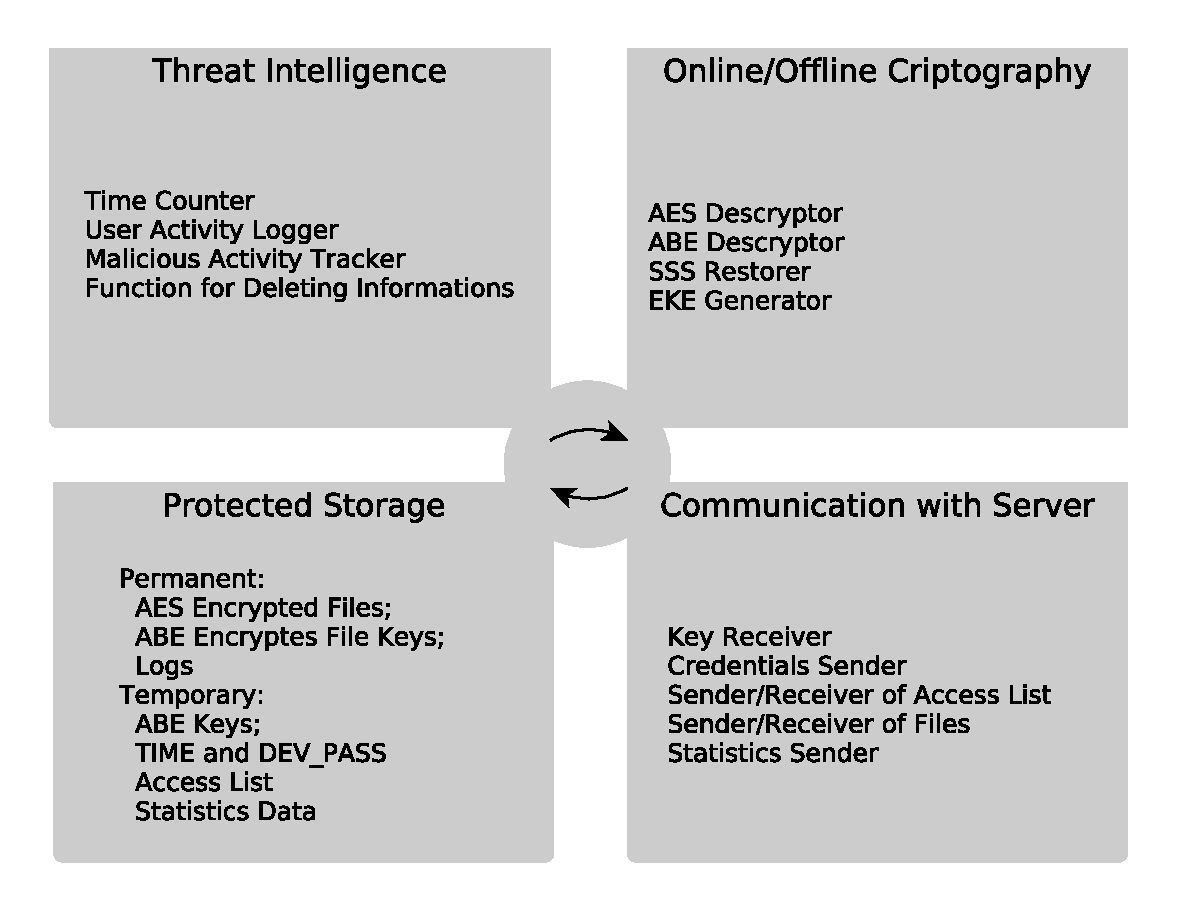
\includegraphics[width=8cm]{figures/fig02.eps}
	\caption{The Mobile Client Architecture}
	\label{fig:02}
\end{figure}

This architecture consists of the modules of cryptographic functions, threat intelligence infrastructure, communication with server and storage.

The cryptographic functions include the decryption (for AES and ABE) key restoration for SSS and EKE token generation procedure. While the AES-ABE hybrid encryption scheme functions both in the online and offline modes, the SSS is used only in the offline mode, while the EKE generation and executions is used in the online mode. These operations are described in Subsections \ref{sec_aes}-\ref{sec_secret} and are part of the Figure \ref{fig:01}.

The threat intelligence infrastructure takes into account simple actors such as the time counter for the key expiry period, the counter of unsuccessful tries in order to protect from brute force attacks, and MOS-inspired statistics analyzer. Functions such as alerting and deleting the expired key belong to this block as well. These functions are described in Subsection \ref{sec_mos}.

The communication with server includes the separate sender and receiver to check the user credentials and receive new keys, which acts based on the EKE protocol. The remaining data like access list and files can be sent via unprotected channels. 

\section{The proposed solution for offline mobile security}
\label{sec_offline_mode}
This section proposes an approach for the mobile client protection in which the security is supported both in online and offline modes. Currently and to the best of our knowledge, the systems of mobile client protection follow a model where the protected client can operate only when it is connected to the cloud, which is not always convenient for the end-user. The basic principles of the mobile client protection herein proposed are: 

\begin{enumerate}
	\item Optimized communication with the cloud when the mobile client does not need to be constantly connected to the server due to the resource constraint and necessity to secure this communication;
	\item Optimized combination of the security mechanisms so that the mobile client does not need to perform complex computation like encryption and key generation due to its resource constraint;
	\item Behavioral analysis of user's operations on mobile client, which can indicate anomalous or automated activities performed by attackers.
\end{enumerate}

The most important security issues in the proposed model arise when the client goes to the offline mode and the user is still allowed to get the access to the protected SME documents. In this case, the server can neither monitor the user activity nor provide the protection methods. The security should be performed at the mobile client. Additionally, the maximum protection should be provided at the minimum resource cost. 

In the online mode the mobile client uses the secure communication with the server in order to verify the validity of user’s credentials. On the contrary, the offline protection model should be approached independently. Thus, the proposal is that the authentication/authorization mechanisms in the offline mode should utilize the derived proof of the user identity. The requirements for the proof are as follows:

\begin{enumerate}
	\item The proof is derived from the previous session, in order to verify that the user is still authorized;
	\item The proof should not give access to user password, i.e. it should not be stored on the app;
	\item The proof should be temporary and have an expiration period;
	\item It should not be directly used in communication with the server, in order to prevent the malicious user from mimicking;
	\item It should be resilient to offline dictionary attacks;
	\item It has to stay effective both in the scenarios of the malicious outsider and leakage of information when the formerly authorized user leaves the group.
\end{enumerate}

Such proof cannot be stored on the client, as it is not possible to guarantee its protection in the offline mode. Therefore, the most effective way to secure the proof on the offline mode without performing complex computation is to share this proof between the mobile client and the user in a protected manner. In this case, there is no need to store the function of the user password. The additional argument against the traditional password verification is the necessity to check the PIN, which is very small, so the construction of valid one-way function resilient to the offline dictionary attacks is difficult.

The proposed architecture for offline mobile security is represented in Figure \ref{fig:03}.

\begin{figure}[h!]
	\centering
	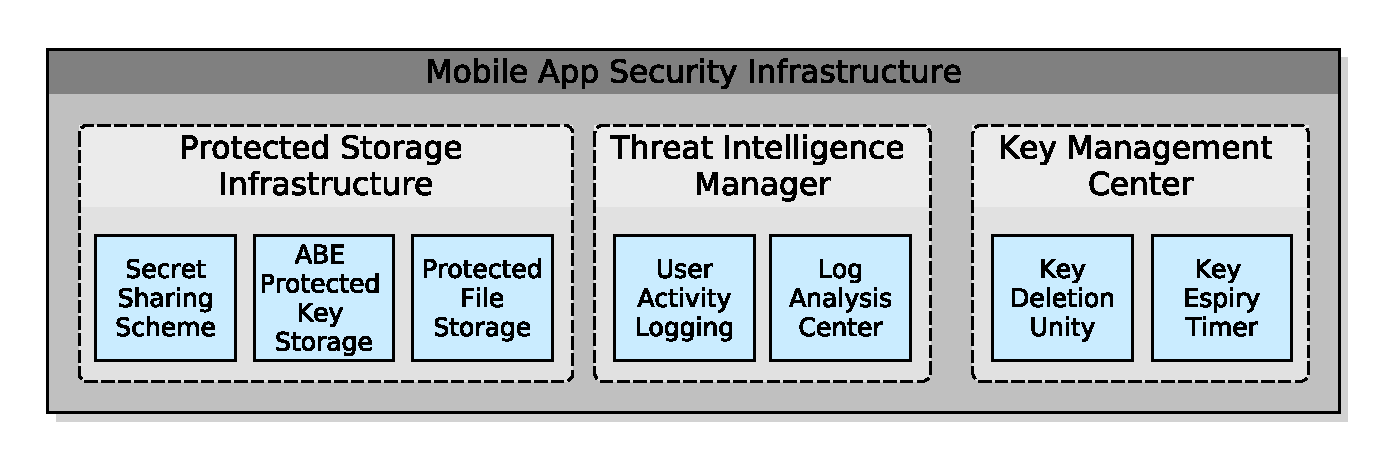
\includegraphics[width=8cm]{figures/fig03.eps}
	\caption{Proposed Architecture for Offline Mobile Security}
	\label{fig:03}
\end{figure}

The Figure \ref{fig:03} describes the proposed architecture for offline mobile security, showing the modules responsible for securing the mobile client, which includes:

\begin{enumerate}
	\item \textbf{Protected Storage}: the storage is protected with the shared user key and contains the ABE keys giving access to the file keys which allow decrypting the stored files. The outline of the hybrid encryption scheme is presented in the Section \ref{sec_algorithms}.
	\item \textbf{Threat Intelligence Manager (TIM)}: most attacks incur into significant variation on the legitimate behavior of information systems, or they adopt well-known patterns that can be easily detected by monitoring the system in the case of the offline mode. Signal processing techniques have been successfully applied to anomaly detection \cite{lu2009network, huang2009signal} and have become a solution to a problem of improving detection accuracy, adaptability and computational cost for application on resource-constrained scenarios. Therefore, signal processing can be applied in offline mobile client security, for evaluating anomalies on user's behavior, according to the scenarios in Section \ref{sec_results}. Moreover, Model Order Selection (MOS), which is an effective signal processing technique to separate noise components from the principal components, can be applied into anomaly and attack detection \cite{tenorio2013greatest}, to identify and separate malicious behaviors from the legitimate ones. The TIM is an internal module of the mobile client that implements offline anomaly detection through signal processing techniques.
	\item \textbf{Key Management Center}: it includes the functions for maintaining the key expiry period and deleting the expired keys. 
\end{enumerate}

\subsection{Offline mode workflow}
\label{sec_offline_mode_workflow}

The user performs the following operations in the offline mode:

\begin{enumerate}
	\item Enters the PASS and the 4-digit PIN;
	\item Views the list of authorized files kept on the mobile storage;
	\item Open the protected encrypted files;
	\item Modify the protected files and save them in an unprotected storage.
\end{enumerate}

The mobile client performs all the cryptographic calculations in the shadow. These calculations include the key storage, key restoring, decryption and showing the decrypted files in the mobile client area. Note that the mobile client does not check the password or PIN validity as it does not hold the verification proof for the above. Also, the mobile client keeps track of the user activities and the key expiry. The complete list of the mobile client activities is presented in the Figure \ref{fig:04}.

\begin{figure}[h!]
	\centering
	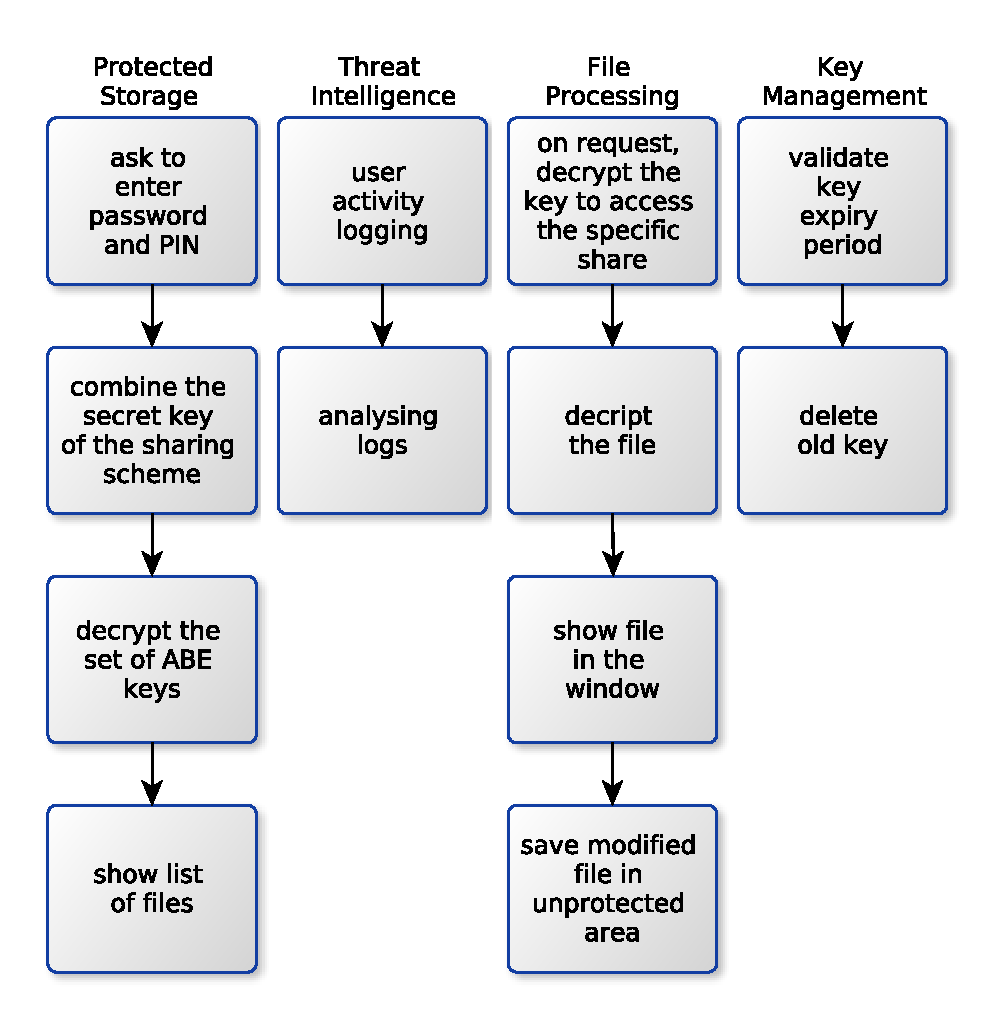
\includegraphics[width=8cm]{figures/fig04.eps}
	\caption{Offline Mode Operations}
	\label{fig:04}
\end{figure}

To finalize the description of the offline mode, Figure \ref{fig:05} shows the complete workflow of the proposed mobile application in the offline-mode.

\begin{figure}[h!]
	\centering
	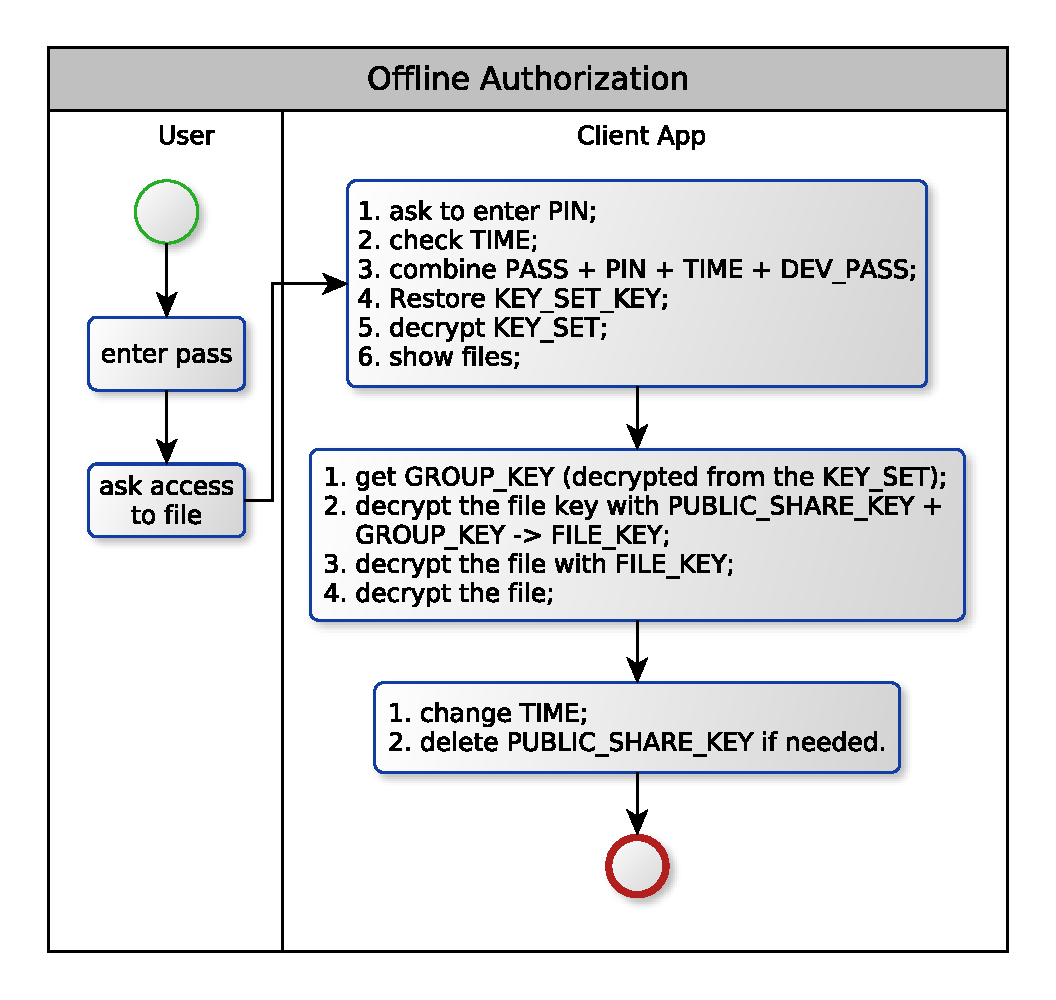
\includegraphics[width=8cm]{figures/fig05.eps}
	\caption{Offline mode authorization workflow}
	\label{fig:05}
\end{figure}

The core cryptographic module of the implemented solution is based on the combination of AES-ABE-SSS methods, described in the Section \ref{sec_algorithms}. The key feature of the offline security is that the mobile client does not actually store any part of the user password to be verified. The mobile client combines its own key with the user share (PIN and password-derived) in order to restore the initial KEY\_SET\_KEY. If the user provides the wrong share the mobile client will not be able to recognize it, but will decrypt the files incorrectly. Additionally, the password entering is tracked and too many tries in a short time are considered a threat.

\subsection{Offline Behavioral Analysis}
\label{sec_offline_behavioral_analysis}

In the proposed client security architecture, the Threat Intelligence Manager (TIM) is responsible for receiving logged user operations, perform feature extraction, data modeling and malicious behavior analysis in order to identify possible threats, in offline mode. Figure \ref{fig:06} depicts the TIM for offline behavioral analysis. 

\begin{figure}[h!]
	\centering
	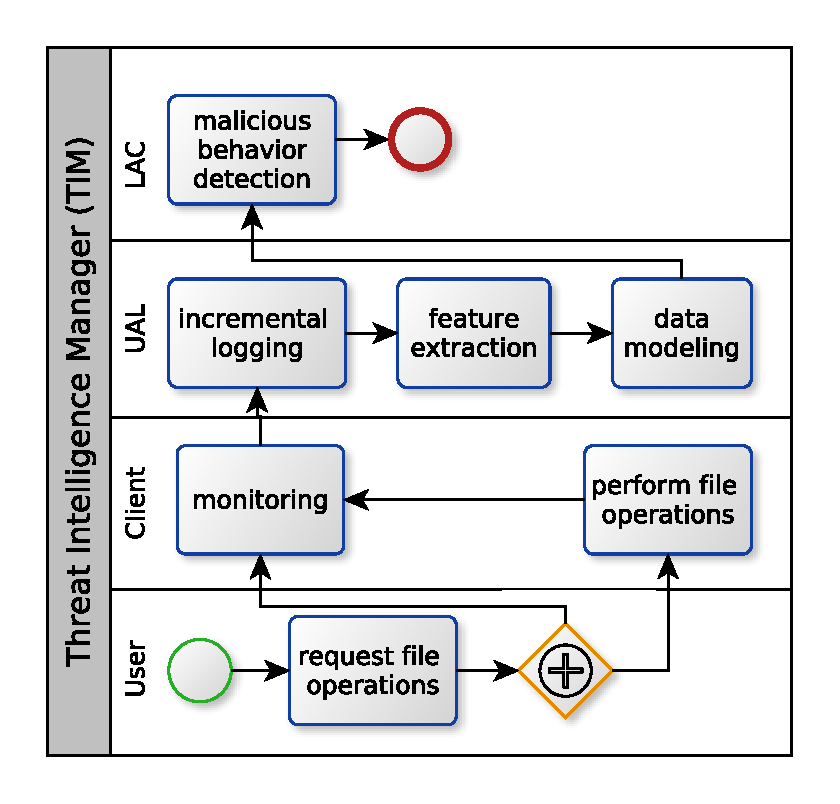
\includegraphics[width=8cm]{figures/fig06.eps}
	\caption{The Threat Intelligence Manager Workflow}
	\label{fig:06}
\end{figure}

As depicted in Figure \ref{fig:06}, users request operations are logged so that the main features can be monitored in the mobile client. The user behavior, trying or effectively executing operations, shall be incrementally captured and logged, making possible to monitor the main features that can reveal malicious behaviors, as well as to identify unexpected behaviors that can reveal possible threats. Therefore, the user operations are monitored by the client app, which sends the information to the User Activity Logging (UAL). 

The UAL is responsible for the incremental logging of activities of the mobile client, feature extraction and data modeling for malicious behavior detection, through the Log Analysis Center (LAC). As an internal module of the mobile client, the UAL implements monitors of selected events of the application, such as a login attempt or a file decryption, and logs the desired information for further analysis. The logged information shall be decomposed into selected features and modeled as matrices, composed of the number of occurrences of the selected features by its location and by time. The resultant data is submitted to the LAC, for anomaly detection.

The LAC performs the behavioral analysis through eigenvalue analysis and MOS schemes, which identify anomalies on sparse, subtle or abrupt number of user operations. The malicious behavior detection is detail described in \ref{sec_mos}.

\section{The algorithms, key usage and data protection methods}
\label{sec_algorithms}
In the proposed approach, the kernel encryption scheme in the mobile client is a combination of several methods of security. The files are encrypted with 128/256-bit AES, while the permanent file keys are encrypted with the attribute-based encryption. The set of expiring ABE keys corresponding to the set of files accessible by user in encrypted with a single expiring AES key (KEY\_SET\_KEY). This key is expiring and is splited by the server into 4 parts (2 are stored on the device and 2 belong to the user) by the method of secure secret sharing. The encryption workflow is outlined in the Figure \ref{fig:07}.

\begin{figure}[h!]
	\centering
	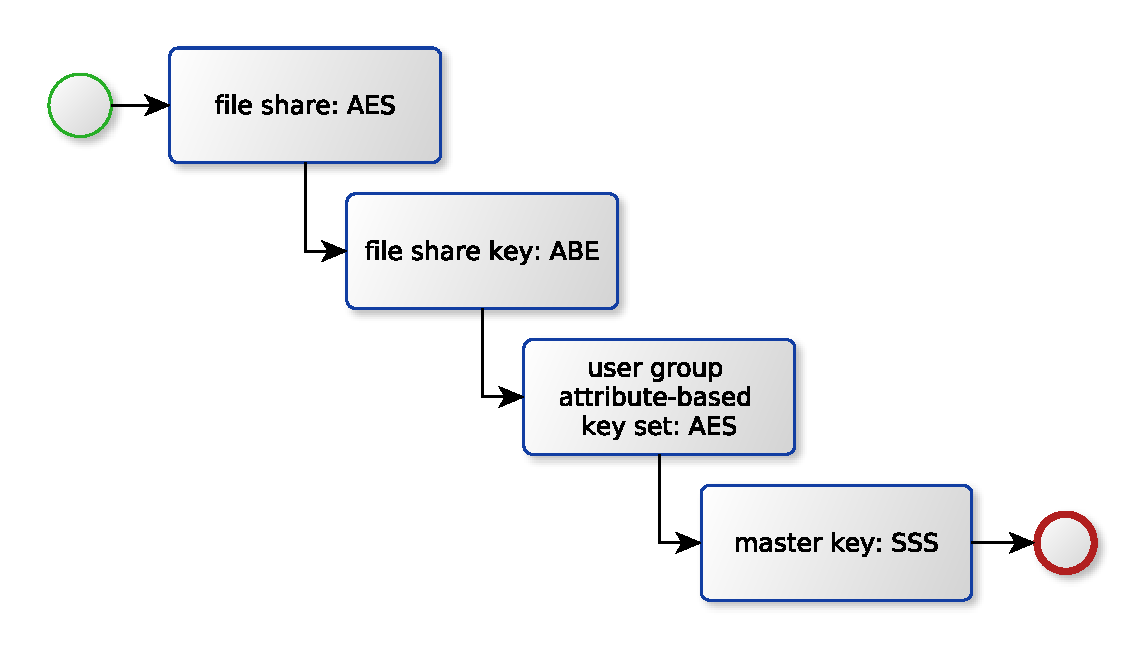
\includegraphics[width=8cm]{figures/fig07.eps}
	\caption{Encryption workflow}
	\label{fig:07}
\end{figure}

The key hierarchy is explained by Figure \ref{fig:08} where the key represented in Figure \ref{fig:07} serves for decrypting the key for each level represented in Figure \ref{fig:08}. As it is possible to be observed in Figure \ref{fig:08}, the master key on the upper level is computed by means of SSS (Subsection \ref{sec_secret}). It serves for decrypting the ABE key storage (section \ref{sec_abe}). The ABE key allows the user finally decrypt the permanent file share keys. Further, the file share can be decrypted by means of AES.

\begin{figure}[h!]
	\centering
	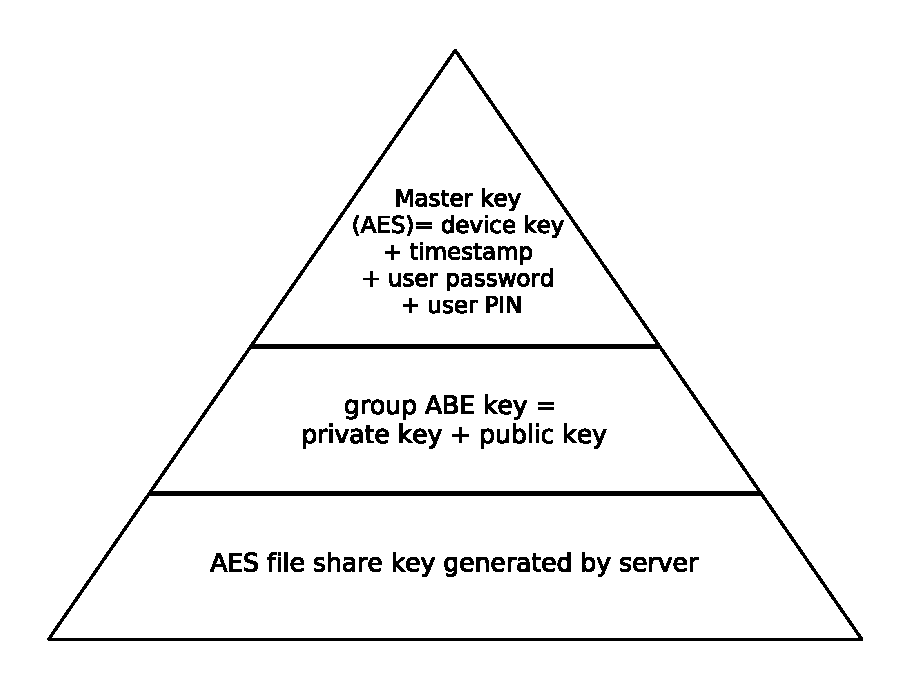
\includegraphics[width=8cm]{figures/fig08.eps}
	\caption{Encryption key hierarchy}
	\label{fig:08}
\end{figure}

This proposed encryption scheme is called as a hybrid encryption since it uses a combination of different encryption methods in order to support all requirements to the encryption scheme used in the proposed infrastructure. Then it has:

\begin{enumerate}
	\item AES provides a fast encryption of the data files;
	\item ABE permits to support the authorization policy on the encryption level;
	\item SSS allows protecting the key storage by avoiding the necessity to store the key proof.
\end{enumerate}

In Subsections \ref{sec_aes}-\ref{sec_secret}, a detailed description of the building blocks of the hybrid encryption is provided, and the proposed malicious behavior detection scheme is detail described in \ref{sec_mos}.

\subsection{AES file encryption }
\label{sec_aes}
The protected files are encrypted on the server side with the secure 128/256 bit AES encryption, which is currently an industrial standard. Nevertheless, it is possible to encrypt the file storage with Blowfish or Serpent which also provide a high level of safety \cite{nist2000}. 

The symmetric encryption on a server side is performed in two steps. First there is a single AES key for preserving the server storage. Second, when the encrypted file is sent from the server to the mobile client another unique AES key is generated, which serves for the encryption on client side. In other words, along with the encrypted file the user gets his own unique AES key for decrypting the files received. This key is protected by attribute-based public key encryption (ABE). 

The scheme of the server-side AES encryption is represented in Figure \ref{fig:09}.

\begin{figure}[h!]
	\centering
	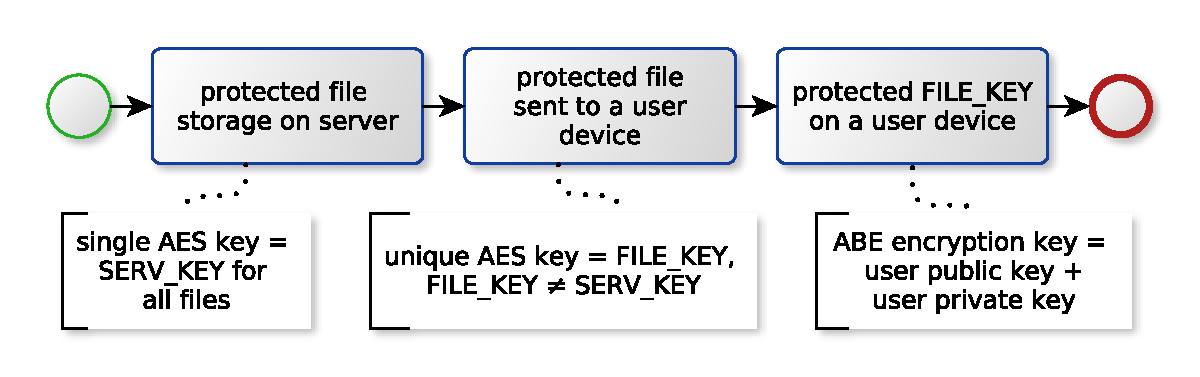
\includegraphics[width=8cm]{figures/fig09.eps}
	\caption{Server-side encryption}
	\label{fig:09}
\end{figure}

Usually, the AES encryption key is used as a session key. In our setting, it is not desirable to re-encrypt the files stored in the device unless there is a certain specific condition (for example, the user leaves the domain or a specific group in the domain (the group of users in the domain contains the users with the equal access rights, i.e. the same set of accessible file shares) and the file should not be accessible for this user anymore). This is why AES key in the presented notation is permanent and defined as FILE\_KEY. The randomly generated FILE\_KEY is unique for each file or set of files stored on a client. 

\subsection{ABE encryption to protect the FILE\_KEY }
\label{sec_abe}
With each user session, the permanent FILE\_KEY (uni\-que AES key) is re-encrypted. The set of FILE\_KEYs is protected with the corresponding ABE keys. The unique ABE model that we propose supports the attribute policy based on user groups and on file shares, i.e. the key attributes correspond both to the groups and the file shares. 

The model supports the simple selective ABE scheme \cite{galibus2015cloud,galibus2014}. The selective scheme for attribute-based encryption is as follows: if at least one attribute in the set $\{t_i\}_U$ is equal to the attribute in the set $\{t_i\}_M$, the corresponding user $U$ can decrypt the text $M$. In other words, as soon as the user and share have one attribute in common – the user can get access to the share. The components of the ABE encryption are:

\begin{enumerate}
	\item \textbf{Master-key (MK)} which is kept safely on server and accessible only for the domain administrator and is given by $MK = (t_1, t_2, \cdots ,t_n, y)$, where the values $t_i$ are randomly selected from the huge group $Zp$. They are the private keys corresponding to the group attributes. Note, that this is different from the usual PK encryption: the private keys are controlled by the admin and not by the users.
	\item \textbf{Public key (PK)} depends on the master key values and is kept in clear allowing users to access the information: $PK = (g^{t_1}, g^{t_2}, \cdots ,g^{t_n}, e(g,g)^y)$. Here $e(g,g)$ is the bilinear pairing function corresponding to an elliptic curve. In order to explain the properties of bilinear paring function, let $\mathbb{G}_1$ and $\mathbb{G}_2$ be two multiplicative cyclic groups of prime order $p$. Let $g$ be a generator of $\mathbb{G}_1$ and $e$ be a bilinear map, $e$: $\mathbb{G}_1 X \mathbb{G}_1 \rightarrow \mathbb{G}_2$. The bilinear map $e$ has two properties, the non-degeneracy, which defines that $e(g,g) \neq 1$, and the bilinearity, which defines that for all $u,v \in \mathbb{G}_1$ and $a,b \in \mathbb{Z}_p$, we have $e(u^a, v^b) = e(u,v)^{ab}$ \citep{goyal2006attribute}. Here $w \in \mathbb{Z}$ is the unique security parameter allowing to control the key generation for each user group.
	\item Secret user \textbf{KEY\_SET} depends on his attribute set. Here each $D_i$ (\textbf{GROUP\_KEY}) serves for decryption of the data of a single group of users, for example, related to some project: 	$\{t_i\}_U \rightarrow D = \{D_i = g^{\frac{yw}{t_i}}\}$.
	\item Encrypted text $M$, in this context, $M = FILE\_KEY$, or the permanent AES symmetric key, which allows to avoid the file re-encryption. The encryption procedure is performed by a multiplication. The set of the public keys $E_i$ (PUBLIC\_SHARE\_KEY) corresponding to the set of groups able to access the text is kept along with the encrypted text $E$: $E=Me(g,g)^{ys}, \{E_i = g^{\frac{t_is}{w}}\}, \forall i, t_i \in \{t_i\}_U$. Here $s \in \mathbb{Z}$ is the unique security parameter allowing to control the key generation for each file share.
	\item Decryption is division: $M = \frac{E}{Y^s}$. 
\end{enumerate}

In order to perform this operation the user needs the pair of private key $D_i$ and public key $E_i$ corresponding to the attribute $t_i$: 

\begin{equation}\label{eq:eq00}
Y^s = e(g,g)^{ys} = e(E_i,D_i) = e(g^{\frac{yw}{t_i}},g^{\frac{t_is}{w}})=e(g,g)^{ys}.
\end{equation}

The result of decryption is the FILE\_KEY - the symmetric AES key that permits to decrypt the contents of protected file. 

\subsection{Secret sharing scheme to protect the key storage }
\label{sec_secret}

The attribute-based private keys $D_i$ should be protected while being stored in the device memory. Therefore, server encrypts the set of $D_i$ with a single AES key before sending it to the user device. This AES key (master key) is denoted by the value KEY\_SET\_KEY in our notation. KEY\_SET\_KEY is a secret value and it is split by the secure method of polynomial modular secret sharing \cite{galibus2015mobile, galibus2008some} into the set of 4 shares: KEY\_SET\_KEY = PASS + PIN + TIME + DEV\_PASS. 

The adversary cannot get any information of the KEY\_SET\_KEY unless he possesses all 4 key parts. Here the values PASS and PIN are predefined similar to the construction in \cite{galibus2015mobile}.

The PASS and PIN values are predefined, similar to the key storing construction based on the polynomial secret sharing scheme (SSS) in \cite{galibus2015cloud}.

In this SSS, the following notation is used: $S(x) \in F_2[x]$ denotes the secret polynomial with coefficients from the finite field $F_2$ to be computed by pooling the shares together. $s_1(x)$, $s_2(x) \in F_2[x]$ denote the shares of the SSS, that are used to compute the secret $s(x)$.

The proposed authentication system is based on the shared storing of the user key. Also, the mobile client acts as a dealer in the SSS. Using the SSS ensures that the key can only be accessed by an authenticated user. The participants of the (2, 2)-threshold SSS are the user and device. The user share $s_1(x)$ is computed based on the PIN and the PASS entered by the user. Additionally, the current time value TIME is used in the calculation of the share. Let $s(x) = d$ and $s_1(x) = f(PIN + PASS + TIME)$, where $f$ is a one-way (hash) function that transforms the data into the string of the desired length: 

\begin{equation}\label{eq:eq01}
  \left\{
  \begin{array}{@{}ll@{}}
    S = s \textrm{ mod } p_0
    \\
    S = s_1 \textrm{ mod } p_1
  \end{array}\right.
\end{equation}

According to the CRT:
\begin{equation}\label{eq:eq02}
S \equiv {s_{1}p_{0}{p_0}^{-1}}_{p1} + {s_{1}p_{1}{p_1}^{-1}}_{p0} + \textrm{ mod } p_0p_1
\end{equation}

Here, $p_0$ and $p_1 \in F_2[x]$ denote the public moduli of the polynomial SSS [10, 11]  and $s \in F_2[x]$ denotes the intermediate secret value. The formulae for these moduli, secret and participants’ shares directly follow from the definition of polynomial SSS construction.

Thus calculated DEV\_PASS is written to the permanent device memory. The user share is not saved. Otherwise, it would allow an attacker to locally validate the restored private key.

\subsection{MOS for Threat Intelligence}
\label{sec_mos}
In the context of anomaly-based schemes for attack detection, the proposed behavioral analysis approach applies signal processing techniques, such as Principal Component Analysis and Model Order Selection schemes \cite{tenorio2013greatest}, for automatic detection of attacks or malicious behaviors. 

Model Order Selection is an effective signal processing technique for several applications, allowing separating the only noise components from the principal components applying a rank reduction of the data. 

Applying MOS to the analysis of user operations can be effective in order to reveal the occurrence of malicious behavior during an offline session. MOS for threat intelligence requires that the target features, which can be user operations, should be modeled as a matrix composed by the number of occurrences by location and time, and grouped into $Q$ time frames. Therefore, the framework considers the time variations of the matrix $\mathbf{X}^{(q)} \in \mathbb{R}^{M\times{N}}$, with $q = 1, \ldots, Q$, in order to detect the occurrence of malicious behaviors. For example, one element of $\mathbf{X}^{(q)}$ can represent the number of file readings on folder $m$ during the minute $n$, from file operations logged by the mobile client.

The MOS schemes can rely on sample covariance of zero mean variables (called as zero mean covariance for the sake of simplicity) and sample covariance of zero mean and unitary standard deviation (called as zero mean and standardized covariance for the sake of simplicity) variables, where the former is useful to identify abnormalities caused by large amounts of operations during a period, while the latter is applied to identify anomalies on sparse or subtle number of file operations.

Classical approaches to model order selection require the computation of the sample covariance matrix $\mathbf{\hat{R}}_{yy}^{(q)}$ and of its eigenvalues, obtained from the measurement matrix $\mathbf{X}$ of the zero mean samples given by

\begin{equation}\label{eq:eq03}
\mathbf{y}_{m}^{(q)} = \mathbf{x}_{m}^{(q)} - \bar{\mathbf{x}}_{m}^{(q)}.
\end{equation}

The set of obtained vectors $\mathbf{y}_{m}^{(q)}$ composes the zero mean matrix $\mathbf{Y}^{(q)}$, then the zero mean covariance matrix $\mathbf{\hat{R}}_{yy}^{(q)}$ can be estimated as follows

\begin{equation}\label{eq:eq04}
\mathbf{\hat{R}}_{yy}^{(q)} = \frac{1}{N}\mathbf{Y}^{(q)}\mathbf{Y}^{(q)^{\rm T}},
\end{equation}
where $\mathbf{\hat{R}}_{yy}^{(q)}$ means the estimation of the sample covariance matrix from the measured zero mean matrix $\mathbf{Y}^{(q)}$ over $N$ minutes of the time frame $q$. 


For MOS based on sample covariance of zero mean and unitary standard deviation, in order to identify anomalies with sparse or subtle behavior, it is required, for each variable, to make the standard deviation unitary as follows

\begin{equation}\label{eq:eq05}
\mathbf{z}_{m}^{(q)} = \frac{\mathbf{x}_{m}^{(q)} - \bar{\mathbf{x}}_{m}^{(q)}}{\mathbf{\sigma}_{m}^{(q)}}.
\end{equation}

The set of vectors $\mathbf{z}_{m}^{(q)}$ composes the matrix $\mathbf{Z}^{(q)}$, then the zero mean and standardized covariance matrix $\mathbf{\hat{R}}_{zz}^{(q)}$ can be calculated via 

\begin{equation}\label{eq:eq06}
\mathbf{\hat{R}}_{zz}^{(q)} = \frac{1}{N}\mathbf{Z}^{(q)}\mathbf{Z}^{(q)^{\rm T}}.
\end{equation}

Once the $\mathbf{\hat{R}}_{yy}$ or $\mathbf{\hat{R}}_{zz}$ have been obtained for MOS in order to anomaly detection, for the sake of simplicity, we refer to $\mathbf{\hat{R}}_{yy}$ or $\mathbf{\hat{R}}_{zz}$ as a matrix $\mathbf{C}$. Therefore, the next step of the algorithm is the eigenvalue decomposition (EVD), calculated according to $\mathbf{C}^{(q)} = \mathbf{V}^{(q)}\mathbf{\Lambda}^{(q)}\mathbf{V}^{(q)^{\rm T}}$, in order to obtain the vector of eigenvalues $e$, as following:

\begin{equation}\label{eq:eq07}
\mathbf{e}^{(q)} = \rm diag(\mathbf{\Lambda}^{(q)}),
\end{equation}

The eigenvalues should be sorted in descending order, as defined by $\lambda_{1}^{(q)} > \lambda_{2}^{(q)} > \lambda_{3}^{(q)} > \cdots > \lambda_{m}^{(q)}$, to make possible the selection of the first eigenvalue in the obtained sequence, represented by $\lambda_{1}^{(q)}$, which is the largest eigenvalue of the data evaluated for attack detection.

The process of obtaining the $\mathbf{X}^{(q)} \in \mathbb{R}^{M\times{N}}$ and the matrix $\mathbf{C}^{(q)}$, finding the largest eigenvalue for each $q$-th time frame, should be repeated until $q = Q$, in order to obtain the largest eigenvalue of all time frames, as presented by 

\begin{equation}\label{eq:eq08}
\mathbf{E} =
\begin{bmatrix}
  \lambda_1^{(1)} & \lambda_1^{(2)} & \lambda_1^{(3)} & \cdots & \lambda_1^{(Q)} \\
  \lambda_2^{(1)} & \lambda_2^{(2)} & \lambda_2^{(3)} & \cdots & \lambda_2^{(Q)} \\
  \lambda_3^{(1)} & \lambda_3^{(2)} & \lambda_3^{(3)} & \cdots & \lambda_3^{(Q)} \\
  \vdots & \vdots & \ddots & \vdots  \\
  \lambda_m^{(1)} & \lambda_m^{(2)} & \lambda_m^{(3)} & \cdots & \lambda_m^{(Q)} \\
\end{bmatrix}.
\end{equation}

Since $\lambda_1^{(q)} > \lambda_2^{(q)} > \lambda_3^{(q)} > \cdots > \lambda_{m-1}^{(q)} > \lambda_m^{(q)}$, then the first line of the matrix $\mathbf{E}$ contains the largest eigenvalues of each $q$-th time frame, which is the expected input for MOS schemes and can be expressed as 

\begin{equation}\label{eq:eq09}
\boldsymbol{e}_{\rm max} = \boldsymbol{E}\{:,1\} = [ \lambda_1^{(1)}, \lambda_1^{(2)} \cdots \lambda_1^{(Q)}]
\end{equation}

Once obtained the largest eigenvalues of each $q$-th time frame, it is possible to apply a selected MOS scheme to estimate the model order $\hat{d}$, which is the estimated number of time frames with malicious behavior. Therefore, $\boldsymbol{e}_{\rm max}$ is used as input parameter for MOS schemes, according to the equation

\begin{equation}\label{eq:eq09}
\hat{d} = \textrm{MOS}(\boldsymbol{e}_{\rm max})
\end{equation}

Note that some MOS schemes may also require the amount of time that compose a time frame, such as $\hat{d} = \textrm{MOS}(\boldsymbol{e}_{\rm max}, M)$. For more information about MOS schemes, interested readers are referred to \cite{da2009comparison}.

\section{Results and analysis}
\label{sec_results}

This section provides the detailed analysis of the results the proposed approach regarding security and complexity analysis.

\subsection{Security analysis}
\label{sec_sec_analysis}
The security analysis of the proposed model was performed both from the point of implemented cryptographic mechanisms and from the user behavioral analysis. Two common attack scenarios were analyzed. First, the malicious outsider trying to infect or steal the important files. Second, the malicious expired user trying to steal the important files. 

\subsubsection{Adversary model}
\label{sec_adversary_model}
The proposal is to use a restricted adversary model. In other words, the actions of the adversary are predicted within the outlines model and scenarios. For example, it is not possible to guarantee the security of the decrypted document once the user copies its content to another file. 

In the analyzed scenarios, it is assumed that the adversary can:

\begin{enumerate}
	\item Steal the user keys one-by-one while the mobile client performs decryption, if the attacker is outsider;
	\item Use expired key to decrypt the files, if the attacker is insider;
	\item Steal the encrypted files.
\end{enumerate}

It is also assumed that the adversary can not:

\begin{enumerate}
	\item Perform offline dictionary attack and cryptanalysis, i.e. does not have the possibility to verify user credentials apart from entering them in the mobile client;
	\item Steal the decrypted files.
\end{enumerate}

\subsubsection{Security analysis}
\label{sec_sec_analysis}

In the offline mode the mobile client does not store the user password (see Section \ref{sec_offline_mode_workflow} for details), i.e. no information about the password leaks, and therefore there is no possibility for the malicious user to check if the password he is trying to enter is correct or not. The possible scenario for the information leakage in the case of the malicious outsider is if:

\begin{enumerate}[label=(\alph*)]
	\item The hacker steals all the parts of KEY\_SET\_KEY;
	\item The hacker steals the KEY\_SET;
	\item The hacker try the brute force offline dictionary attack on all the previous values, they have to belong to ONE TIME SESSION (the values of ”a” and ”b” belong to one period of time i.e. TIME, DEV\_PASS, KEY\_SET);
	\item Steal the permanent FILE\_KEY (this is protected by the KEY\_SET);
	\item Steal the file and try to decrypt it with offline dictionary attacks.
\end{enumerate}

Still, the hacker has to get 4 values from one session: TIME, DEV\_PASS, KEY\_SET, FILE\_KEY. At the same time he should try the offline dictionary attack on PIN+PASS. Moreover, the 4 values provide access only to 1 single file. So practically, it is very difficult to perform such attack due to the key expiration period. In accordance with the conditions 1 and 3 of our adversary model, the above actions are not possible for such adversary in the conditions presented.

The temporary nature of all parameters obliges the user to connect to server when necessary and prevents the malicious actions from the user side. The possible scenario when malicious or expired user wishes to prolong his old credentials is:

\begin{enumerate}[label=(\alph*)]
	\item Steal the file and try to decrypt it with offline dictionary attacks.
	\item He has to be able to combine;
	\item He has to steal the KEY\_SET synchronized with his credentials;
	\item He has to steal the protected FILE\_KEY (also synchronized) and encrypted file;
	\item He has to do everything without the mobile client (because the client checks the TIME and renews the PUBLIC\_SHARE\_KEY).
\end{enumerate}

Basically, for a malicious user there is practically no way to use the mobile client with the old keys. The fact that the client does not contain any data to be checked or validated does not prevent the user from seeing the contents of decrypted files, but with the wrong password the decrypted files will be different from the original ones.

The mobile client still has to count the tries (to prevent the hacker to perform brute force attack) within one session. In accordance with the conditions 2 and 4 of the adversary model, the above actions are not possible for such adversary.

\subsubsection{Common threat scenarios}
\label{sec_common}
This section provides the detailed description of the common scenarios in which the log and behavioral analysis is provided. The behavioral analysis can help to keep the user or administrator informed of the threat and take actions, as well as it can be useful in order to implement threat preventions or reactive actions to avoid threat propagation.

\begin{thm}
An attacker uses a valid password to perform operations on a bulk of files.
\end{thm}

The session time defines the period when operations can be performed until the next session renewing. During this period, it is still necessary to identify attacks and malicious behavior on file operations, in order to avoid fast attacks to perform unauthorized access to information or data modification. Some attacks present behavioral patterns based on abrupt number of operations, such as the ransomware attack, which is a growing attack \cite{McAfee2015} that blocks the access to valuable resources and requires a payment in order to unblock the content. The access to the resources can be blocked by the attacker through some techniques, when the content is encrypted by the attacker, the ransomware attack can be called cryptoransomware \cite{kaspersky2014}.

MOS schemes based on zero mean covariance analysis are effective to reveal abrupt changing of behaviors over time \cite{tenorio2013greatest}, making possible to identify intense malicious behaviors on offline mode of mobile clients, such in case of ransomware attack or bulk access to sensitive data.

The large number of operations over time is a well-known pattern of some attacks, due to the efforts on security measures to make the attacks infeasible over time. In this context, the operations can also be evaluated in contrast to the estimated required time for operations done by legitimate behaviors, such as the evaluation of the mean time between operations, highlighting the occurrence of infeasible behaviors in comparison to legitimate user activities.

Sparse or subtle file operations, with low number of operations distributed over different files or directories, during short period of time can indicate anomalies in contrast to the required time for legitimate directory navigation. MOS and zero mean and standardized covariance analysis can be suitable if applied to evaluate the time and location of operations, in order to identify unreachable navigation, if compared to legitimate navigation

The MOS based on zero mean covariance analysis indicates abnormalities caused by large amounts of operations during a period. Subsequently, the eigenvalue analysis highlights massive or concentrated operations over time or folder location, which is evaluated by MOS schemes in order to identify the number of malicious behaviors during the evaluated time.

This threat scenario, where an attacker uses a valid password and session to perform operations on a bulk of files, can have its steps described as:

\begin{enumerate}[label=(\alph*)]
	\item The hacker has access to the mobile client and is able to perform operations;
	\item The session time is valid;
	\item The hacker tries to perform legitimate operations, such as file decryption, encryption, reading, writing or directory navigations;
	\item The mobile client incrementally append each operation attempt time into the logging;
	\item The MOS module evaluates the logging of legitimate operations, applying zero mean and standardized covariance analysis to identify anomalies on sparse or subtle number of file operations, highlighting the occurrence of infeasible behaviors in comparison to legitimate user activities;
	\item The MOS module evaluates the logging of legitimate operations, applying zero mean covariance analysis to identify abnormalities caused by massive operations during the session time.
\end{enumerate}

\begin{thm}
Usage of expired password to perform unauthorized operations.
\end{thm}

In the offline mode, the session time is used to restrict the operations during a specified period, although it is possible to manipulate the current time in mobile device, to emulate a period in which the session was valid. The log analysis by MOS can deal with this kind of threat, through the incremental logging of the time when each operation was performed, followed by the behavioral evaluation of operations over time. 

The incremental logging assumes that new logged operations shall have equal or bigger time than the last logged operation, the violation of this rule means that the system is out of sync and indicates a malicious behavior. Additionally, a large amount or sparse operation performed at the same time, or during a short period, can indicate the use of backtrack techniques to maintain a valid session during necessary time to perform an attack. Massive, subtle or sparse malicious operation performed during a valid session time can be identified by MOS schemes based on covariance analysis.

Applying MOS to the analysis of the time between user operations can be effective in order to reveal the occurrence of malicious behavior during an offline session. The MOS based on zero mean and standardized covariance analysis identifies anomalies on sparse or subtle variation in the number of file operations, since the eigenvalue analysis highlights the unexpected number of sparse (such as file operations on diverse folders) or subtle operations. Consequently, the result of the eigenvalue analysis is applied to MOS schemes, in order to identify the occurrence of malicious behaviors during the valid session.

The MOS based on zero mean covariance analysis indicates abnormalities caused by large amounts of operations during a period. The eigenvalue analysis based on the zero mean covariance matrix highlights massive or concentrated operations over time or location, which is evaluated by MOS schemes in order to identify the number of malicious behaviors during the evaluated time.

This threat scenario, where the attacker uses expired password to perform unauthorized operations, can have its steps described as:

\begin{enumerate}[label=(\alph*)]
	\item The hacker steals the operating system;
	\item The hacker modifies the time of the operating system to a period when the session was valid;
	\item The hacker has access to the mobile client and is able to perform operations;
	\item The hacker tries to perform legitimate operations, such as file decryption, encryption, reading, writing or directory navigations;
	\item The mobile client incrementally append each operation attempt time into the logging;
	\item The mobile client verifies if one logged time is older than the last operation time. If it is true, the MOS module classifies the evaluated operation as malicious;
	\item The MOS module evaluates the logging of legitimate operations, applying zero mean and standardized covariance analysis to identify anomalies on sparse or subtle number of file operations;
	\item The MOS module evaluates the logging of legitimate operations, applying zero mean covariance analysis to identify abnormalities caused by massive operations during the session time;
\end{enumerate}

\subsubsection{Data Modeling for Behavioral Analysis }
\label{sec_data}

MOS schemes are used in order to identify anomalous behavior that can indicate an attack and be used to prevent or avoid attack propagation. Therefore, it is necessary to analyze the data that can be collected from user operations on mobile client, to identify features that can be modeled and submitted to MOS schemes, according to described in Section \ref{sec_mos}.

The selected features shall be modeled as matrices which represents a signal superposition containing noise, legitimate and malicious behavior \cite{tenorio2013greatest}, grouped into time frames $\mathbf{X}^{(q)} \in \mathbb{R}^{M\times{N}}$, with $q = 1, 2, 3, \ldots, Q$ , where $M$ defines the decomposition of a selected feature, $N$ defines the time decomposition and represents the number of occurrences of the feature $m$ during the time $n$.

In offline mode, the user is still allowed to get access to operations that do not require communication with the server side. These operations and their selected features shall be incrementally logged by the UAL of the mobile client, in order to be analyzed by the TIM to identify malicious behaviors. 

This work proposes to evaluate the following features, which represents events of the user operating the mobile client.

\paragraph{\textbf{File Access (Time and File System Location)},}i.e. data access to selected files in offline mode, accessing the data stored on the mobile client. The file access feature can be decomposed into more detailed features, which are:

\begin{enumerate}
	\item file decryption; 
	\item decrypted file reading;
	\item decrypted file execution. 
\end{enumerate}

Therefore, it is necessary to generate three matrices for the following malicious behaviors analysis: 

\begin{enumerate}[label=(\alph*)]
	\item massive file access, which can reveal data leakage and be identified by MOS schemes based on zero mean covariance analysis; 
	\item low file access into several folders, characterized by sparse operations that can reveal unreachable navigation performed by automated file accesses in order to avoid the massive file access characterization;
	\item Malicious sparse file accesses can be identified by MOS schemes based on zero mean and standardized covariance analysis. 
\end{enumerate}

\paragraph{\textbf{File Update (Time and File System Location)},}i.e. writing operations into selected files in offline mode, writing the data stored on the mobile client. The update feature can be decomposed into:

\begin{enumerate}
	\item file encryption;
	\item decrypted file writing.
\end{enumerate}

Therefore, it is necessary to generate two matrices for malicious behaviors analysis, such as: 

\begin{enumerate}[label=(\alph*)]
	\item massive file update, which can reveal ransomware or similar attacks and be identified by MOS schemes based on zero mean covariance analysis; 
	\item low number of file update into several folders, characterized by sparse operations that can reveal unreachable navigation performed by automated file accesses in order to avoid the massive file access characterization. Malicious sparse file accesses can be identified by MOS schemes based on zero mean and standardized covariance analysis.
\end{enumerate}

\paragraph{\textbf{File Download (Start Time, End Time and File System Location)},}i.e. download requests in online mode, evaluated by the mobile client. The file download feature shall be modeled as the matrix of number downloads by file location over time, in order to perform malicious behaviors analysis, such as:

\begin{enumerate}
	\item massive data leakage or similar attacks, which can be identified by MOS schemes based on zero mean covariance analysis;
	\item low number of file download from several folders, characterized by sparse operations, which can reveal unreachable navigation performed by automated file download in order to avoid the massive file download characterization. Malicious sparse file download can be identified by MOS schemes based on zero mean and standardized covariance analysis.
\end{enumerate}

\paragraph{\textbf{File Upload (Start Time, End Time and File System Location)},}i.e. upload requests in online mode, evaluated by the mobile client. The file upload feature can reveal attempts of ransomware or similar attacks and be identified by MOS schemes based on covariance analysis. Therefore, it is necessary model the matrix of number uploads by file location over time, in order to perform malicious behaviors analysis, such as:

\begin{enumerate}
	\item massive file upload, similar to ransomware attack, which can be identified by MOS schemes based on zero mean covariance analysis; 
	\item low number of file upload to several folders, characterized by sparse operations, which can reveal unreachable navigation performed by automated file upload in order to avoid the massive file upload characterization. Malicious sparse file upload can be identified by MOS schemes based on zero mean and standardized covariance analysis.
\end{enumerate}

\begin{table*}[!t]
	\caption{Speed of decryption on a client device}
	\label{tab:01}
	\centering
	\begin{tabular}{|l|l|l|l|l|l|}
		\hline \rowcolor{Gray} Device Model	& File set size	& \begin{tabular}[x]{@{}l@{}}Mean time of\\getting decrypted\\stream (ABE)\end{tabular}	& \begin{tabular}[x]{@{}l@{}}Mean time of\\decrypting \\content (AES)\end{tabular}	& \begin{tabular}[x]{@{}l@{}}Mean time of\\copying file\\without decrypt\end{tabular}	& \begin{tabular}[x]{@{}l@{}}Mean time of\\decryption\\(the whole file)\end{tabular}	\\ \hline

		\begin{tabular}[x]{@{}l@{}}SM-T320 Galaxy Tab Pro 8.4\end{tabular}	& 10 mb	& 1041 ms	& 4230 ms	& 298 ms		& 5271 ms	\\ \hline
		\begin{tabular}[x]{@{}l@{}}SM-T320 Galaxy Tab Pro 8.4\end{tabular}	& 1 mb	& 811 ms		& 319 ms		& 23 ms		& 1130 ms	\\ \hline
		\begin{tabular}[x]{@{}l@{}}SM-T320 Galaxy Tab Pro 8.4\end{tabular}	& 1 kb	& 1078 ms	& 1 ms		& 0 ms		& 1080 ms	\\ \hline
		\begin{tabular}[x]{@{}l@{}}GT-I9190 Galaxy S4 Mini\end{tabular}		& 1 b	& 1167ms		& 2 ms		& 0 ms		& 1169 ms	\\ \hline
		\begin{tabular}[x]{@{}l@{}}GT-I9190 Galaxy S4 Mini\end{tabular}		& 1 kb	& 1141ms		& 2 ms		& 0 ms		& 1144 ms	\\ \hline
		\begin{tabular}[x]{@{}l@{}}GT-I9190 Galaxy S4 Mini\end{tabular}		& 1 mb	& 1138 ms	& 368 ms		& 35 ms		& 1506 ms	\\ \hline
		\begin{tabular}[x]{@{}l@{}}GT-I9190 Galaxy S4 Mini\end{tabular}		& 10 mb	& 1131 ms	& 3618 ms	& 324 ms		& 4750 ms	\\ \hline
	\end{tabular}
\end{table*}

\begin{table*}
	\caption{Speed of receiving the list of files}
	\label{tab:02}
	\centering
	\begin{tabular}{|l|l|l|l|l|l|l|l|l|l|}
		\hline \rowcolor{Gray} \begin{tabular}[x]{@{}l@{}}Files\\quantity\end{tabular}	 	& Samples 	& \begin{tabular}[x]{@{}l@{}}Average\\(ms)\end{tabular}	 	& \begin{tabular}[x]{@{}l@{}}Min\\(ms)\end{tabular}	& \begin{tabular}[x]{@{}l@{}}Max\\(ms)\end{tabular} 	& Std. Dev. 	& Error (\%)		& Throughput 	& KB/sec 	& Avg. Bytes \\ \hline
		1		& 1000	& 131	& 29		& 321	& 31.56		& 0.00\%		& 74		& 161.32		& 2233	\\ \hline		
		10		& 1000	& 154	& 37		& 269	& 32.24		& 0.00\%		& 63.4	& 659.79		& 10656	\\ \hline
		100		& 1000	& 396	& 68	 	& 1055	& 87.56		& 0.00\%		& 25		& 2323.2		& 95308	\\ \hline
		1000		& 1000	& 2879	& 475	& 4634	& 496.02		& 0.00\%		& 3.4	& 3178		& 946311	\\ \hline
	\end{tabular}
\end{table*}

\begin{table*}
	\caption{Speed of generating the user keys}
	\label{tab:03}
	\centering
	\begin{tabular}{|l|l|l|l|l|l|l|l|l|}
		\hline \rowcolor{Gray} Label	& Samples	& \begin{tabular}[x]{@{}l@{}}Average\\(ms)\end{tabular}	& \begin{tabular}[x]{@{}l@{}}Min\\(ms)\end{tabular}	& \begin{tabular}[x]{@{}l@{}}Max\\(ms)\end{tabular}	& Std. Dev.	& Throughput		& KB/sec		& Avg. Bytes \\ \hline
		\begin{tabular}[x]{@{}l@{}}Login 5 shares available\end{tabular}		& 1000	& 982	& 225	& 1990	& 271.88		& 20.1	& 146.36		& 7459	\\ \hline
		\begin{tabular}[x]{@{}l@{}}Login 10 shares available\end{tabular}	& 1000	& 1140	& 340	& 4176	& 459.3		& 17.3	& 223.88		& 13218	\\ \hline
		\begin{tabular}[x]{@{}l@{}}Login 25 shares available\end{tabular}	& 1000	& 1267	& 887	& 2303	& 192.75		& 15.5	& 294.55		& 19466 \\ \hline
	\end{tabular}
\end{table*}

\subsection{Complexity analysis}
\label{sec_complex}

\begin{table*}
	\caption{Data Modeling and Eigenvalue Decomposition Time }
	\label{tab:04}
	\centering
	\begin{tabular}{|l|l|l|l|l|l|l|l|}
		\hline \rowcolor{Gray} Device	& \begin{tabular}[x]{@{}l@{}}Log Size\\(MB)\end{tabular}	& \begin{tabular}[x]{@{}l@{}}Window\\(min)\end{tabular}	& \begin{tabular}[x]{@{}l@{}}Modeling\\(ms)\end{tabular}	& \begin{tabular}[x]{@{}l@{}}Avg. Eig.\\(ms)\end{tabular}	& \begin{tabular}[x]{@{}l@{}}Std. Eig.\\(ms)\end{tabular}	& \begin{tabular}[x]{@{}l@{}}Eig. Min.\\(ms)\end{tabular}	& \begin{tabular}[x]{@{}l@{}}Eig. Max.\\(ms)\end{tabular}	\\ \hline
		Galaxy GT-I9300	& 6	& 60	& 107	& 209.52	& 18.58	& 183	& 276	\\ \hline
		Galaxy GT-I9300	& 6	& 40	& 115	& 227.26	& 18.13	& 191	& 289	\\ \hline
		Galaxy GT-I9300	& 6	& 20	& 89	& 268.14	& 21.94	& 229	& 315	\\ \hline
		Galaxy GT-I9300	& 6	& 10	& 90	& 347.42	& 24.11	& 304	& 421	\\ \hline
		Galaxy GT-I9300	& 4.1	& 60	& 20	& 60.90	& 15.19	& 37	& 106	\\ \hline
		Galaxy GT-I9300	& 4.1	& 40	& 20	& 68.72	& 15.71	& 43	& 114	\\ \hline
		Galaxy GT-I9300	& 4.1	& 20	& 34	& 89.04	& 16.78	& 54	& 133	\\ \hline
		Galaxy GT-I9300	& 4.1	& 10	& 21	& 117.24	& 14.36	& 96	& 171	\\ \hline
		Galaxy GT-I9300	& 1.4	& 60	& 10	& 159.82	& 15.82	& 125	& 197	\\ \hline
		Galaxy GT-I9300	& 1.4	& 40	& 10	& 168.06	& 15.90	& 139	& 220	\\ \hline
		Galaxy GT-I9300	& 1.4	& 20	& 11	& 204.4	& 20.46	& 176	& 269	\\ \hline
		Galaxy GT-I9300	& 1.4	& 10	& 13	& 259.00	& 21.34	& 220	& 315	\\ \hline
		Galaxy Tab SM-T800	& 6	& 60	& 7	& 59.30	& 6.55	& 54	& 74	\\ \hline
		Galaxy Tab SM-T800	& 6	& 40	& 8	& 62.56	& 7.05	& 56	& 80	\\ \hline
		Galaxy Tab SM-T800	& 6	& 20	& 10	& 73.28	& 8.59	& 65	& 95	\\ \hline
		Galaxy Tab SM-T800	& 6	& 10	& 8	& 93.48	& 9.13	& 83	& 130	\\ \hline
		Galaxy Tab SM-T800	& 4.1	& 60	& 11	& 18.64	& 4.51	& 16	& 38	\\ \hline
		Galaxy Tab SM-T800	& 4.1	& 40	& 11	& 19.64	& 5.12	& 17	& 38	\\ \hline
		Galaxy Tab SM-T800	& 4.1	& 20	& 12	& 25.12	& 5.55	& 21	& 46	\\ \hline
		Galaxy Tab SM-T800	& 4.1	& 10	& 12	& 32.32	& 7.29	& 27	& 55	\\ \hline
		Galaxy Tab SM-T800	& 1.4	& 60	& 4	& 49.08	& 6.01	& 42	& 62	\\ \hline
		Galaxy Tab SM-T800	& 1.4	& 40	& 5	& 51.42	& 7.36	& 44	& 74	\\ \hline
		Galaxy Tab SM-T800	& 1.4	& 20	& 5	& 51.12	& 7.80	& 54	& 91	\\ \hline
		Galaxy Tab SM-T800	& 1.4	& 10	& 7	& 75.24	& 7.71	& 65	& 90	\\ \hline
	\end{tabular}
\end{table*}

The complexity analysis depends on the operation that the user and the mobile client perform in order to keep the app protected. In the offline mode the mobile client performs the following actions:

\begin{enumerate}
	\item Combine the PASS + PIN + TIME + DEV\_PASS = KEY\_SET\_KEY $\rightarrow$ SSS secret restoring;
	\item Decrypt the KEY\_SET with the KEY\_SET\_KEY $\rightarrow$ symmetric 128/256 AES decryption;
	\item Select the SHARE\_KEY from the KEY\_SET $\rightarrow$ no calculation;
	\item Decrypt the FILE\_KEY with the SHARE\_KEY $\rightarrow$ ABE decryption;
	\item Decrypt the file with the FILE\_KEY $\rightarrow$ symmetric 128/256 AES $\rightarrow$ decryption;
	\item Modify the TIME periodically $\rightarrow$ timer;
	\item Count the tries within the TIME $\rightarrow$ count;
	\item Modify or delete PUBLIC\_SHARE\_KEY $\rightarrow$ no calculation;
	\item Malicious behavior detection $\rightarrow$ eigenvalues calculation.
\end{enumerate}

It is easy to check that in the offline mode the mobile client does not perform complex calculations and does not use the resources extensively due to the fact that the initial key is shared and the mobile client only performs decryption, which is not a time-consuming operation. Thus, the proposal supports the concept of the light-weighted client, i.e. the most consuming actions are ABE and AES decryption. 

Similarly, in the online mode the mobile client does not perform resource-consuming actions apart from J-PAKE construction which is used to renew the user/app master key (DEV\_PASS):

\begin{enumerate}
	\item Generates keys for J-PAKE $\rightarrow$ this can be a resource-consuming action. In the future we suggest to replace J-PAKE with SIS-based PKE \cite{bogos2013primeless,bellovin1992encrypted};
	\item Sends and receives data in the clear;
	\item Performs actions 1)-7);
	\item Performs the action 8) and sends the log data for server side analysis.
\end{enumerate}

The proposed concept of mobile client security has been implemented in the Storgrid protected cloud environment \cite{storgrid2016}. Therefore, the approach is correlated with the practical usability requirements: the corporate user continues to use the mobile storage app in offline and does not need to reload the files every time the key is renewed. This methodology can be used in other mobile clients. The common advantage is that the mobile client performs the operations both in the offline and online mode and uses the key expiry and ABE to protect the privacy of the corporate data. 

Table \ref{tab:01} presents the results of mobile client security workflow testing and demonstrates that the proposed scheme decrypts the data with acceptable speed. One can compare the speed of ABE/AES decryption (keys and actual data) and the speed of the whole decryption process.

Table \ref{tab:02} demonstrates the results of testing the speed of the mobile client for receiving and displaying the list of files. The client was tested for displaying up to 1000 files. Around 100 requests were generated from 10 threads. It is possible to observe that the client receives and displays the list of files depending on the user attributes with acceptable average speed, showing that the proposed protection scheme is usable. 

Table \ref{tab:03} demonstrates the results of performance testing of the keys generation procedure on server. It is possible to observe that the performance does not decrease drastically with the increase of particular user shares. Each key sample generated contains the domain member code, key data and the sharing key value for each file sharing code. It is possible to conclude that the proposed client is not overloaded with calculations due to the carefully selected mathematical operations. It can be successfully used and provides acceptable level of security.

The log analysis of the Log Analysis Center (LAC) has been implemented and evaluated for offline anomaly detection in mobile clients, making it possible to apply anomaly detection techniques in a lightweight fashion, considering low processing requirements for deal with the resource constraints of mobile clients. The evaluation considered the required processing time for anomaly detection from log analysis, measuring the data modeling time through the UAL, the eigenvalue decomposition time and the required time for the EDC MOS scheme execution, which is the scheme that requires less processing capacity and provides more anomaly identification accuracy \cite{da2009comparison,tenorio2013greatest}. 

The experiments were performed in two mobile devices, Galaxy GT-I9300 and Galaxy Tab SM-T800, with variations of log size and window size. The Galaxy GT-I9300 has Quad-core 1.4 GHz Cortex-A9 processor and 1 GB RAM, while the Galaxy Tab SM-T800 has its processing capacity composed by Quad-core 1.9 GHz Cortex-A15 and quad-core 1.3 GHz Cortex-A7, and 3 GB RAM.

Table \ref{tab:04} presents the data modeling time and the processing time of eigenvalues decomposition calculations to be applied to anomaly detection from user operation logs of Storgrid mobile client. The information presented by column are the device model, the log size in megabytes, the window size in minutes, the data modeling time in milliseconds, the average of eigenvalue decomposition time in milliseconds, the standard deviation of eigenvalue decomposition time in milliseconds, the minimum of eigenvalue decomposition time in milliseconds and the maximum of eigenvalue decomposition time in milliseconds.

The results show that the lower window size leads to the larger eigenvalue decomposition time, but the largest eigenvalue decomposition time, which was the maximum of 421 milliseconds with average of 347.42 milliseconds. This result highlights an acceptable speed even for the worst evaluated scenario, which is the case using a Galaxy GT-I9300 for processing 6MB with window size of 10 minutes.

\begin{table*}[!t]
	\caption{EDC MOS scheme processing time for anomaly detection}
	\label{tab:05}
	\centering
	\begin{tabular}{|l|l|l|l|l|l|l|l|}
		\hline \rowcolor{Gray} Device	& \begin{tabular}[x]{@{}l@{}}Log Size\\(MB)\end{tabular}	& \begin{tabular}[x]{@{}l@{}}Window\\(min)\end{tabular}	& \begin{tabular}[x]{@{}l@{}}Avg. EDC.\\(ms)\end{tabular}	& \begin{tabular}[x]{@{}l@{}}Std. EDC.\\(ms)\end{tabular}	& \begin{tabular}[x]{@{}l@{}}Min. EDC.\\(ms)\end{tabular}	& \begin{tabular}[x]{@{}l@{}}Max. EDC.\\(ms)\end{tabular}	\\ \hline
		Galaxy GT-I9300	& 6	& 60	& 5.27	& 4.04	& 3	& 20	\\ \hline
		Galaxy GT-I9300	& 6	& 40	& 10.78	& 6.37	& 6	& 34	\\ \hline
		Galaxy GT-I9300	& 6	& 20	& 32.62	& 12.44	& 21	& 88	\\ \hline
		Galaxy GT-I9300	& 6	& 10	& 115.08	& 17.45	& 88	& 158	\\ \hline
		Galaxy GT-I9300	& 4.1	& 60	& 5.68	& 4.18	& 3	& 23	\\ \hline
		Galaxy GT-I9300	& 4.1	& 40	& 10.76	& 5.31	& 7	& 27	\\ \hline
		Galaxy GT-I9300	& 4.1	& 20	& 37.58	& 10.30	& 23	& 61	\\ \hline
		Galaxy GT-I9300	& 4.1	& 10	& 125.98	& 18.56	& 101	& 191	\\ \hline
		Galaxy GT-I9300	& 1.4	& 60	& 4.92	& 3.49	& 3	& 17	\\ \hline
		Galaxy GT-I9300	& 1.4	& 40	& 9.00	& 4.23	& 6	& 25	\\ \hline
		Galaxy GT-I9300	& 1.4	& 20	& 30.14	& 9.21	& 19	& 62	\\ \hline
		Galaxy GT-I9300	& 1.4	& 10	& 100.62	& 15.83	& 69	& 163	\\ \hline
		Galaxy Tab SM-T800	& 6	& 60	& 1.84	& 0.65	& 1	& 3	\\ \hline
		Galaxy Tab SM-T800	& 6	& 40	& 3.26	& 1.24	& 2	& 7	\\ \hline
		Galaxy Tab SM-T800	& 6	& 20	& 10.90	& 2.40	& 9	& 21	\\ \hline
		Galaxy Tab SM-T800	& 6	& 10	& 41.86	& 7.33	& 34	& 60	\\ \hline
		Galaxy Tab SM-T800	& 4.1	& 60	& 1.85	& 0.60	& 1	& 3	\\ \hline
		Galaxy Tab SM-T800	& 4.1	& 40	& 3.62	& 1.10	& 2	& 8	\\ \hline
		Galaxy Tab SM-T800	& 4.1	& 20	& 12.04	& 2.79	& 9	& 22	\\ \hline
		Galaxy Tab SM-T800	& 4.1	& 10	& 40.16	& 6.48	& 35	& 60	\\ \hline
		Galaxy Tab SM-T800	& 1.4	& 60	& 1.98	& 0.89	& 1	& 6	\\ \hline
		Galaxy Tab SM-T800	& 1.4	& 40	& 3.30	& 1.16	& 2	& 7	\\ \hline
		Galaxy Tab SM-T800	& 1.4	& 20	& 10.48	& 2.90	& 8	& 21	\\ \hline
		Galaxy Tab SM-T800	& 1.4	& 10	& 34.52	& 4.08	& 30	& 45	\\ \hline
	\end{tabular}
\end{table*}

Table \ref{tab:05} presents the processing time of EDC MOS calculations applied to anomaly detection from user operation logs of Storgrid mobile client. Table \ref{tab:05} respectively presents the device model, the log size in megabytes, the window size in minutes, the average of EDC calculation time in milliseconds, the standard deviation of EDC calculation time in milliseconds, the minimum of EDC calculation time in milliseconds and the maximum of EDC calculation time in milliseconds.

It is possible to observe that the processing time increases with the window size decreasing, similar to the results for eigenvalue decomposition time. The longest processing time measured is lower than 200 milliseconds, even considering window size of 10 minutes or processing 6 MB of user operation log. This result represents an acceptable processing time for anomaly detection in mobile clients.

\section{Conclusion and future work}
\label{sec_conclusion}

An important security issue faced by corporations that use cloud-based systems is how to provide security mechanisms to support offline corporate mobile clients. Once a mobile client releases the connection with the corporate cloud, no security measure implemented in the cloud infrastructure assures the protection of sensitive data stored in the mobile device. Aware of this problem and its importance, this work presented a proposal to address the offline mobile security problem combining a different cryptographic methods. Moreover, this proposed approach also prevents malicious user behavior by applying a MOS-based analytic method. 

As prove of concept, a fully working mobile application was developed to test the proposed security solution and acquired results provide evidence that besides achieving the desired security features, the solution also has positive results in terms of performance. This fact is due to the usage of lightweight operations and the optimized combination of the selected security methods. The proposed approach is a practical application to be used in the corporate mobile environment. It is implemented as a fully working mobile client and can be used for any type of enterprise. Also, part of concept is seed for new security solutions for big data apps. 

Future works in the area can further explore enhancements in the analytics methods as well as to extended the approach to be used by mobile devices with even more severe resources constraints.